\chapter{Architettura del sistema}
\label{ch:architecture}
Il \textit{Progetto Velocity} è una parte di un sistema di Track\&Trace il cui scopo è il monitoraggio in near real time della logistica.
Al momento il sistema monolitico legacy gestisce tutto, il nuovo sistema, il cui primo componente è \textit{Velocity}, lo soppianterà gradualmente, seguendo un approcio \textit{brownfield}.
In questo momento si stanno sviluppando i nuovi servizi e li si sta integrando con il vecchio sistema, i nuovi clienti vengono direttamente gestiti con le componenti
funzionanti del nuovo sistema, i clienti che invece venivano gestiti con il sistema legacy stanno venendo gradualmente trasferiti.

\section{Sistemi coinvolti}
\label{sec:architecture_entity}

\begin{figure}[H]
\centering
    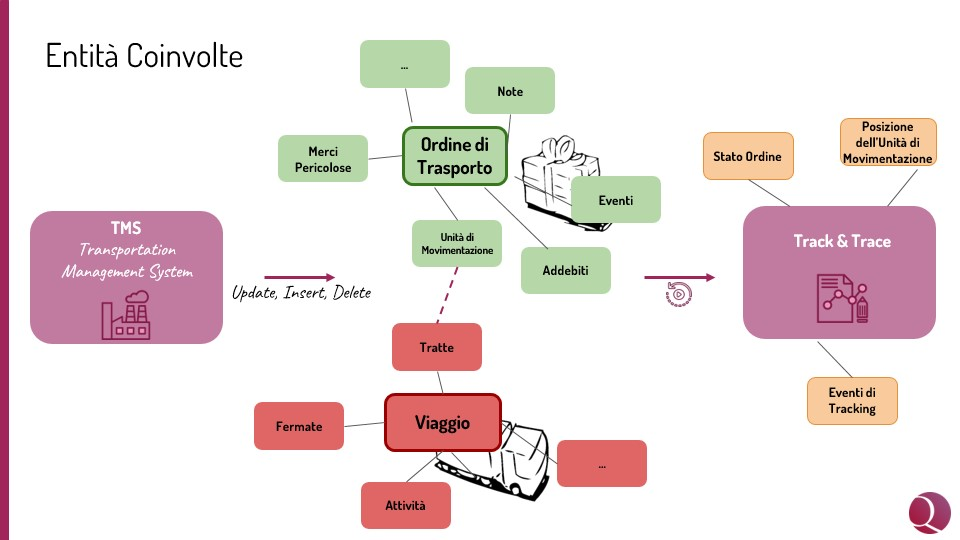
\includegraphics[width=\textwidth]{images/architecture/entita_coinvolte.jpg}
    \caption{Entità coinvolte}
    \label{fig:architecture_entities_img}
\end{figure}

La sorgente dei dati è il \textit{Transport Management System (TMS)} un software esterno che effettua modifiche a diverse entità.
Con il termine \textbf{Entità} si intende qualsiasi caratteristica che definisce un oggetto o situazione reale, ad esempio un \textit{viaggio} potrebbe avere le seguenti entità:
\textit{origine,destinazione, durata, etc ...}\\
Nel sistema le entità sono raggruppabili in diversi domini, i cui 3 principali sono:
\begin{itemize}
    \item Ritiro
    \item Ordine di trasporto (Spedizione)
    \item Viaggio
\end{itemize}
In figura \ref{fig:architecture_entities_img} sono presentati due domini d'esempio, \textit{Viaggio} e \textit{Ordine di Trasporto}.
I vari domini non sono isolati l'uno dall'alto, bensì la modifica di una entità potrebbe implicare la modifica di un'altra entità.
In figura \ref{fig:architecture_entities_img} ad esempio modificando una \textit{unità di movimentazione} verrebbe conseguentemente modificata una \textit{tratta}.
\\
\\
Lo scopo del sistema \textbf{Velocity} è proprio quello di tenere traccia di tutti i cambiamenti subiti dalle varie entità (effettuati dal \textbf{TMS}).
Ciò avviene tramite \texttt{Debezium} (sezione \ref{sec:debezium_overview}) che monitora i database del \textbf{TMS} generando eventi di dominio, che verranno poi processati da altri microservizi.
%nel video quello che io chiamo entità vengono chiamati "root aggregate", anzi ancora diverso. sono tutte entità, ma le entità "viaggio" o "ordine trasporto" sono dei Root Aggregate, cioè degli oggetti che si portano dietro molte altre informazioni.
Il \textbf{T\&T} si occupa anche di fornire ai clienti informazioni sullo stato e sulla storia di diversi oggetti, composti dalle entità.
Ad esempio potrebbe essere fornito l'oggetto \textit{Carico} che descrive lo spostamento di un mezzo e tutte le consegne effettuate,
quindi costituito da \textit{Tratta e Fermate} ma anche dalle informazioni riguardo alle merci che trasporta, cioè \textit{Note,Unità di movimentazione, etc ...}

\section{Track and Trace legacy}
\label{sec:T&T_old}
Lo scopo del sistema di \textbf{Track \& Trace}  è quello di fornire al cliente tracciabilità sugli ordini da lui effettuati.
Ciò può risultare di limitata importanza se si pensa ad un cliente finale, ma quando si tratta di un cliente business,
che potrebbe necessitare di consegne per iniziare o proseguire lavorazioni, la tracciabilità diventa un requisito fondamentale.
Il \textbf{T\&T} è una funzionalità già presente nel \textit{TMS}, però questi non genera tutti gli eventi che servono,
nasce quindi la necessità di avere un software che calcoli questi eventi mancanti, partendo da quelli che il TMS genera e da eventuali fonti esterne (ad esempio le comunicazioni con i camion). 
Esempio concreto: il TMS genera gli eventi "ordine creato" e "camion partito", ma non genera l'evento "ordine spedito". 
Andando ad analizzare quali sono gli ordini che sono stati caricati sul camion, il \textit{T\&T} è in grado di generare l'evento "ordine spedito" per ognuno di essi.
\\\\
Il \textbf{Track \& Trace legacy} è un software monolitico che gestisce tutto, dalle modifiche agli oggetti di business alla comunicazione con il cliente, basato su batching e non orientato ad eventi.
Essendo un sistema basato su Batch, a regolari intervalli di tempo va a vedere il nuovo stato delle entità ed aggiorna un suo database interno di oggetti composti.
L'idea alla base della migrazione in microservizi è quindi quella di partizionare il vecchio sistema monolitico e renderlo basato su microservizi ed ad eventi.
I vantaggi di creare un sistema orientato ad eventi sono due:
\begin{itemize}
    \item Il sistema reagisce prontamente agli eventi, senza dover aspettare che un batch venga eseguito.
    \item Il sistema intercetta tutti gli eventi, anche quelli intermedi. Ad esempio se un ordine viene creato e poi annullato, il sistema monolitico non si accorge di nulla, se queste due operazioni avvengono nell'intervallo tra l'esecuzione di una batch e l'altra. 
\end{itemize}
Quindi sono state prese alcune responsabilità del vecchio sistema e le si sono spostate in un nuovo sistema (\textit{Velocity}) basato su eventi.
Altre fuzionalità sono invece state implementate in un nuovo sistema, che attinge da Velocity e svolge le restanti funzioni del \textit{T\&T}.
Al momento ci sono quindi due sistemi di \textit{T\&T}, uno alimentato da velocity, l'altro completamente indipendente.
I due sistemi \textit{T\&T} sono sviluppati in \texttt{.NET}, il vecchio è un servizio Windows che gira su un server virtuale, 
il nuovo è una \texttt{Azure function} (simili alle AWS lambda), che si trova sul cloud Azure ed è in ascolto sui \textit{Kafka topic} su cui opera \textit{Velocity}.
\\\\
Velocity presenta una limitazione, lavorando con approccio \textit{Brownfield} deve interfacciarsi con i vecchi sistemi, sia in input che in output.
L'input arriva dal \textit{TMS} e per renderlo compatibile viene usato \texttt{Debezium} (sezione \ref*{sec:debezium_overview}) in modo da leggere dal suo db.
In output invece il problema è che \textit{Velocity} non implementa tutte le funzionalità del vecchio sistema, ma solo una parte.
In particolare la fase finale di comunicazione con i clienti (invio di email, aggiornamento del portale web, etc..) non è implementata in Velocity,
Quindi \textit{T\&T} (quello alimentato da velocity) è completamente identico al vecchio \textit{T\&T}, ma senza le feature che adesso sono gestite da \textit{Velocity}

\section{Project Velocity}
\label{sec:project_velocity}
Lo scopo del progetto \textit{Velocity} è costruire un \textit{T\&T} il più veloce possibile.
Prima dell'implementazione ad eventi il tempo necessario alla ricezione da parte del cliente dell'aggiornamento di un'ordine era di 40 minuti.
In seguito all'introduzione di \textit{Velocity} questo tempo è sceso a 5 minuti, con l'implementazione dell' \texttt{EventExport} \ref{cap:MicroservizioEventExport} l'obbiettivo è portarlo a meno di 3.
Per rendere possibile ciò Il progetto è completamente ad eventi, basato su \texttt{Apache Kafka} \ref{ch:kafka_overview}. 
Inoltre per ridurre al minimo la latenza il sistema è costruito su una architettura cloud, che per il momento si appoggia ad \texttt{Azure} ed è pensata apposta per essere scalabile.
\begin{figure}[H]
    \centering
    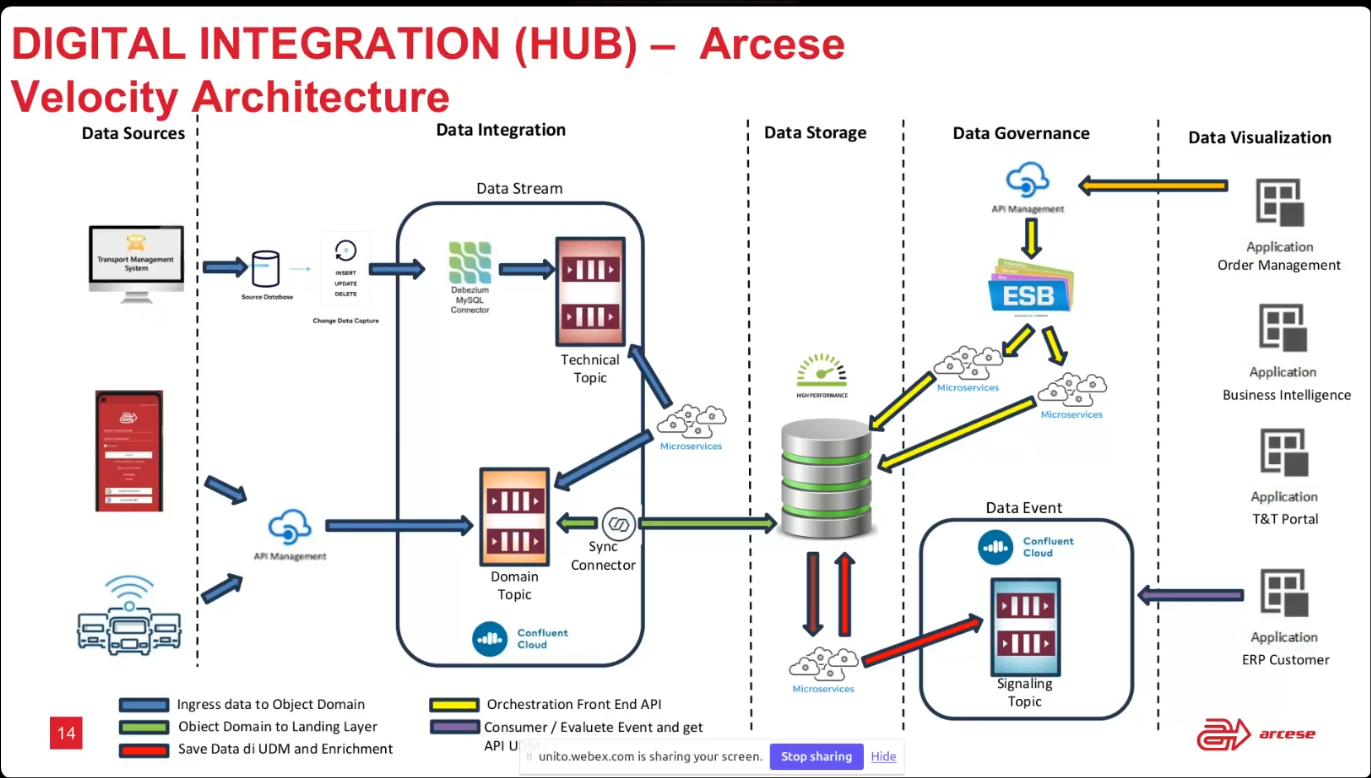
\includegraphics[width=\textwidth]{images/architecture/collocazione_velocity.png}
    \caption{Collocazione di Velocity}
    \label{fig:collocazione_velocity_img}
\end{figure}
TODO: chiedere a Massimo se è possibile avere la slide.
l'Immagine \ref{fig:collocazione_velocity_img} è mostrato dove si colloca \textit{Velocity} all'interno del sistema.
\textit{Velocity} (quello che in nell'immagine vede etichettato come "confluent cloud") lavora con input che arrivano dal \textit{TMS}, cioè con \textbf{Technical Events},
oppure con input che arrivano dagli autisti dei camion tramte apposita app interna, cioè con \textbf{Business Events}.
La differenza tra questi due eventi sarà approfondita nella sezione \ref{sec:velocity_streams}.


\subsection{Streams usati da Velocity}
\label{sec:velocity_streams}
\textit{Velocity} è un sistema \textit{Event Driven} basato su \texttt{Kafka Streams}. (sezione \ref{subsubsec:kafka_stream})
Quando una entità cambia stato la modifica viene registrata su un \texttt{Kafka Topic} e, successivamente, gli eventi sui Topic vengono analizzati o filtrati tramite \texttt{Kafka Stream}.
Possiamo distinguere 3 tipologie di \texttt{Kafka Topic}:
\begin{figure}[H]
    \centering
    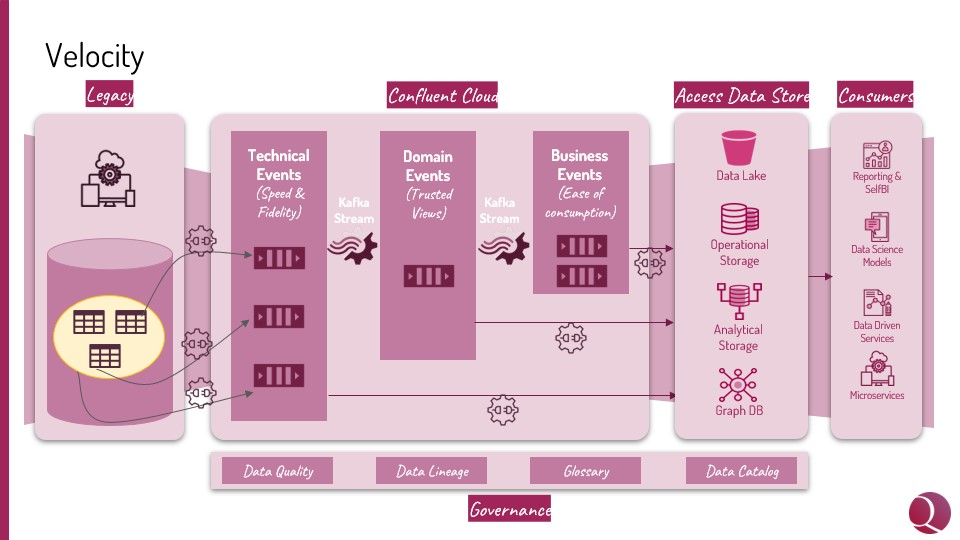
\includegraphics[scale=0.5]{images/architecture/confluent_velocity.jpg}
    \caption{Tipologie di Kafka Topics}
    \label{fig:kafka_topics.img}
\end{figure}
\begin{itemize}
    \item \textbf{Technical Events, Technical Topic }: Contengono gli eventi generati dal \textbf{TMS}, sono eventi molto simili a dei log di un database
    (essendo generati tramite \texttt{Debezium} sono sostanzialmente una collezione di operazioni SQL) e spesso sono ridondanti, è
    infatti comune che il sistema effettui operazioni poco efficienti.
    Ad esempio qualora io avessi un ordine con una nota e la volessi modificare il TMS potrebbe svolgere la richiesta segnalando una operazione di \texttt{DELETE} ed una di \texttt{INSERT} piuttosto che effettuare una semplice \texttt{UPDATE}.\\
    É presente un \texttt{Topic} di tipo \textit{Technical Events} per ogni tabella del database originale (quindi un topic ogni dominio).
    \item \textbf{Domain Events, Domain Topic}: Questi Topic contengono gli eventi filtrati dai \textit{Technical Events} tramite i \texttt{Kafka Streams} 
    e gli eventi generati dai corrieri tramite una applicazione interna ad Arcese.
    Non sono più simili a dei log di un DB (già solo la loro struttura è JSON, non SQL) e rappresentano come è fatto un oggetto (ordine di trasporto, viaggio, ...). 
    Tutti i potenziali eventi ridondanti sono stati filtrati dallo \textit{Stream}, non vi è più quindi il problema degli eventi ridondanti.
    \item \textbf{Business Events, Signaling Topic}: \texttt{Topic} opzionali, contengono degli eventi strutturati come i consumatori si aspettano (Ease of consumption).
    Sono pensati per fornire una vista specifica per un particolare consumer.
\end{itemize}
Il lavoro svolto nell'ambito della scrittura di questa tesi è stato principalmente concentrato sui \textit{Business Events}, 
dato che il resto del sistema era già stato implementato tramite \textit{Kafka Streams}.
Uno schema generico del funzionamento dei due topic non trattati in seguito si può trovare nella sezione \ref{subsec:components}, insieme all'analisi di due processi
rilevanti che operano sul \textbf{Fast Storage} (mostrato in figura \ref{fig:collocazione_velocity_img}).
Invece i \textit{Business Events} sono trattati nel dettaglio in sezione \ref{subsec:business_events}.

\subsection{Business Events e Signaling Topic}
\label{subsec:business_events}
Al posto di addossare ad un sistema monolitico la responsabilità di trattare i \textit{Business Event},con le difficoltà che ciò comporterebbe,
si è scelto di utilizzare un Kafka Topic su cui scrivere i \textit{Business Event}. 
Il motivo di tale scelta è che i \textit{Business Event} sono molto dipendenti dal consumatore che li leggerà, quindi è meglio fornire una generica interfaccia
e delegare la responsabilità di trattare gli eventi al consumatore.
Inoltre questa loro costruzione li rende perfetti per la logica a microservizi, infatti non è così raro che si voglia modificare un consumer, senza la logica a microservizi
si sarebbe obbligati a cambiare il sistema monolitico per poterlo fare.
Il \textit{Signaling Topic} è ascoltato da diversi microservizi che possono vedere tutti gli eventi, ma processano solo quelli a cui sono interessati e si preoccupano di inoltrarli ai clienti.
Un esempio di microservizio che si occupa di inoltrare gli avvisi di tracciamento ai clienti è \texttt{EventExport} (sezione \ref{cap:MicroservizioEventExport}).
\\\\
come si può vedere in figura \ref{fig:collocazione_velocity_img} i \textit{Business Events} (che vivono nel \textit{Signaling topic}) sono eventi generati dai \textit{Kafka Streams}.
I \textit{Domain Events} che vivono sul \textit{Domain Topic}, vengono elaborati attraverso i \textit{Kafka stream} e vengo scritti nel \textit{Fast Storage}.
Dal fast storage vengono letti ed elaborati da diversi microservizi che arrichiscono ed unificano le informazioni, in seguito vengono scritti nel \textit{Signaling Topic}.
Ad esempio un oggetto di dominio "consegna" porta con se diversi eventi di business: l'aggiornamento della geolocalizzazione dell'ordine ad esso associato, la notifica dell'avvenuta consegna al cliente, etc ...
Basandosi su quanto scritto nel \textit{Fast Storage}, che è stato scritto in base ai \textit{Domain Events} precedentemente giunti al \textit{Domain Topic},
i microservizi che osservano il \textit{Fast Storage} generano \textit{Business Events}.
\\\\
Dato che i consumer che ascoltano il \textit{Signaling Topic} ma processano solo gli eventi a cui sono interessati, 
i Business Events devono essere strutturati in maniera da permettere ai vari consumer di decidere se l'evento è di loro interesse o meno.
Questi eventi perciò contengono 3 principali informazioni:
\begin{itemize}
\item tipo di evento: spedizione, ritiro, viaggio, disposizione o ordine FTL (Full Truck Load)
\item quali oggetti nel datamodel sono stati modificati.
Ciò corrisponde a speficare quali tabelle all'interno del \textit{Fast Storage} sono state interessate dal \textit{Domain Event}.
\item quali "campi sensibili" sono stati modificati.
I campi sensibili sono quei campi che, se modificati, possono interessare il consumer dell'evento.
Ad esempio, se un ordine cambia data di consegna, il consumer (ed il cliente) potrebbero essere molto interessati a questa informazione.
\end{itemize}



\subsection{Componenti}
\label{subsec:components}

\subsubsection{Kafka Streams}
\label{subsubsec:kafka_stream}
\texttt{Kafka Streams} è una API per processare eventi su un \texttt{Topic Kafka} (filtrare, trasformare, aggregare, ...), questo tema viene approfondito nella sezione \ref{subsec:kafka_streams}\\
\\
Gli \texttt{Stream} che collegano i \texttt{Topic} di tipo \textit{Domain Events} a quelli di tipo \textit{Domain Business Event} sono molto dipendenti dalle necessità del consumatore che poi li leggerà quindi non seguono una struttura fissa.
Invece gli \texttt{Stream} che leggono dai \textit{Technical Events Topic} seguono una struttura precisa e svolgono operazioni suddivisibili in 3 fasi:
\begin{enumerate}
    \item \textbf{Fase di Casting}.\\
    In questa fase avviene la ricostruzione dell'evento basandosi sui log generati da \texttt{Debezium} che sta osservando il \textbf{TMS}.\\
    \texttt{Debezium} si occupa di rilevare ogni cambiamento e pubblica l'evento su diversi topic kafka, uno per tabella (quindi uno per ogni dominio). 
    \item \textbf{Fase di Filtro}\\
    Successivamente gli eventi ridondanti devono essere eliminati. Tutti gli eventi relativi ad una transazione vengono accorpati e viene generato un unico evento risultante, che non riporta gli eventi intermedi. 
    \item \textbf{Fase di Mapping}\\
    Il nuovo evento viene quindi trasformato in un \textit{Domain Event} ed inserito sul relativo Topic.
\end{enumerate}

\subsubsection{MicroBatch}
\label{subsubsec:micro_batch}
Questo microservizio si occupa di "ricostruire" una entità a partire da tutti gli eventi che la riguardano. 
Non legge direttamente dal Topic \textit{Domain Events} quindi non è un \textit{consumer Kafka} bensì legge gli eventi di dominio da elaborare da un database SQL chiamato \texttt{Fast Storage}
che viene continuamente aggiornato da un connettore JDBC.
Gli eventi che riceve in input sono quindi dei \textit{Domain Events}, già filtrati dai relativi \texttt{Kakfa Stream}.\\
Dopo la "ricostruzione" l'oggetto viene riscritto nel Fast Storage, eliminando da esso gli eventi che lo riguardavano e che non sono più necessari.
Il microservizio \texttt{MicroBatch} è scritto usando \textit{Spring Batch} e lo scheduler su cui si appoggia per eseguire i Job è \textit{Quartz}.\\\\
Il primo passo, svolto ogni 5 secondi, è un partizionamento. Una classe \texttt{Spring Batch} chiamata \textit{Partitioner} divide gli eventi di dominio in \textit{chunks}, in modo da poterli processare in parallelo.
Il numero di \textit{chunks} è liberamente configurabile, ma il partizionatore è scritto in modo da raggruppare gli eventi con la stessa chiave di dominio (cioè relativi alla stessa Transazione) nella stessa partizione.
Questo non garantisce però che all'interno di un \textit{chunk} ci siano solo eventi con la stessa chiave di dominio.
A questo punto vengono eseguiti i vari \textit{Jobs}, uno per ogni \textit{chunk}, la cui esecuzione si può suddividere in 3 passi.
\begin{enumerate}
    \item \textbf{Reading}: Durante la fase di \textit{Reading} vengono recuperati dal Fast Storage tutti gli Eventi di Dominio che sono stati assegnati dal Partizionatore a quello specifico \textit{chunk}.
    \item \textbf{Processing}: Fase in cui si trasformano gli Eventi di Dominio recuperati durante la fase di \textit{Reading} in una serie di record pronti alla scrittura, ovvero in una serie di oggetti di tipo \texttt{Entity}.
    Le \textit{Entità} andranno quindi a comporre degli oggetti di vario tipo, infatti \texttt{MicroBatch} non si occupa di tenere aggiornata una sola tabella, bensì diverse tabelle sullo stesso database. \todo{quando avro accesso al DB potrò inserire questi esempi}
    Quindi partendo dagli stessi Eventi di Dominio verranno generati diversi record (diverse \texttt{Entity}) che verranno scritti su diverse tabelle.
    \item \textbf{Writing}:Fase finale di scrittura sul Fast Storage. É una scrittura transazionale, quindi deve rispettare le proprietà \texttt{ACID}, requisito di cui si occupa il \textit{Job}.
    Inoltre il \textit{Job} si occupa di verificare per ciascuna tabella se i dati che ha generato devono essere inseriti o solamente aggiornati.
\end{enumerate}

\subsubsection{Event Engine}
\label{subsubsec:event_engine}
Similmente a \texttt{Micro Batch} (sezione \ref{subsubsec:micro_batch}) l'\textit{Event Engine} si occupa di "costruire" degli oggetti di business partendo dal \textit{Fast Storage}, questi oggetti sono pensati per la \textit{ease of consumption} di eventuali client.\\
In altre parole si occupa di osservare i cambiamenti di stato dei diversi eventi di dominio (segnalati dall \textbf{SGA} che monitora il \textbf{TMS}) e generare una serie di eventi di business associati (es: 
“spedizione partita”, “ritiro fallito”, “arrivo stimato”, …)\\\\
Rispetto al caso \texttt{Micro Batch} (\ref{subsubsec:micro_batch})la fase di \textit{Reading} ritorna solo un record per ogni chiave di dominio,
quindi ad ogni \textit{chunk} corrisponde una e solo una chiave di dominio.
Invece le tre altre due fasi (\textit{Processing e Writing}) sono sostanzialmente identiche, con la differenza che la fase di Processing non va a generare un oggetto, bensì calcola una serie di metriche come "orario di partenza", "Tragitto", "Stato dell'ordine", etc ....